\renewcommand*{\arraystretch}{1.1}

\subsection*{BI / read / 23}
\label{section:bi-read-23}

\noindent\begin{tabularx}{\queryCardWidth}{|>{\queryPropertyCell}p{\queryPropertyCellWidth}|X|}
	\hline
	query & BI / read / 23 \\ \hline
%
	title & Holiday destinations
 \\ \hline
%
	pattern & \hfill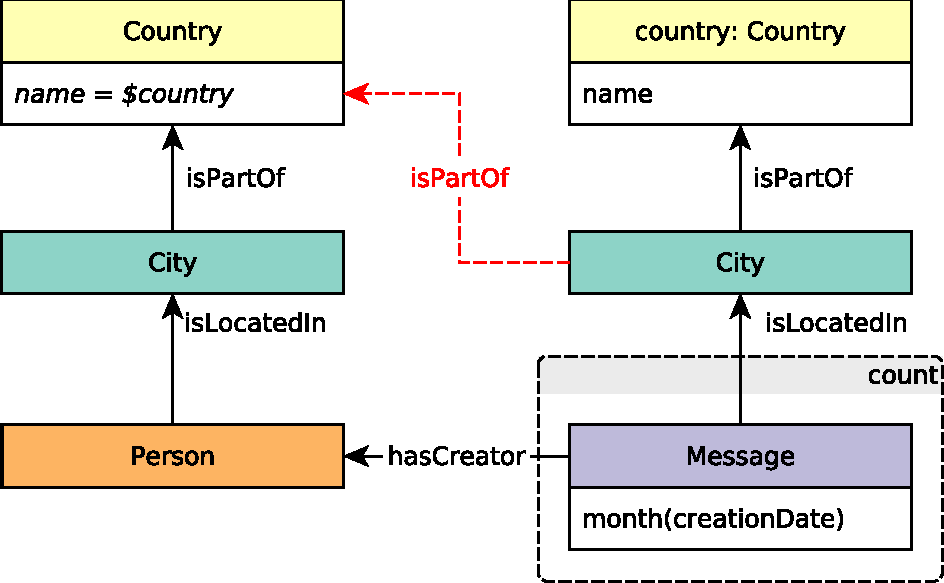
\includegraphics[scale=\patternscale,margin=0cm .2cm]{patterns/bi-read-23}\hfill\vadjust{} \\ \hline
%
	desc. & Count the \emph{Messages} all residents of a given \texttt{country} who
have written a \emph{Message} abroad, grouped by month and Country. A
\emph{Message} was written abroad if the \emph{Country} of the
\emph{Message} was written in is different than the \emph{Country} of
the \emph{Person} it was written by.
 \\ \hline
%
	
		params &
		\innerCardVSpace{\begin{tabularx}{\attributeCardWidth}{|>{\paramNumberCell}c|>{\varNameCell}M|>{\typeCell}m{\typeWidth}|Y|} \hline
		$\mathsf{1}$ & country
 & String
 &  \\ \hline
		\end{tabularx}}\innerCardVSpace \\ \hline
	
%
	
		result &
		\innerCardVSpace{\begin{tabularx}{\attributeCardWidth}{|>{\resultNumberCell}c|>{\varNameCell}M|>{\typeCell}m{\typeWidth}|>{\resultOriginCell}c|Y|} \hline
		$\mathsf{1}$ & messageCount
 & 32-bit Integer
 & R &
				The number of \emph{Messages} in each group
 \\ \hline
		$\mathsf{2}$ & country.name
 & String
 & R &
				The name of the destination \emph{Country}
 \\ \hline
		$\mathsf{3}$ & month
 & 32-bit Integer
 & R &
				 \\ \hline
		\end{tabularx}}\innerCardVSpace \\ \hline
	
%
	
		sort		&
		\innerCardVSpace{\begin{tabular}{|>{\sortNumberCell}c|>{\varNameCell}l|>{\directionCell}c|} \hline
		$\mathsf{1}$ & messageCount
 & $\desc
$ \\ \hline
		$\mathsf{2}$ & country.name
 & $\asc
$ \\ \hline
		$\mathsf{3}$ & month
 & $\asc
$ \\ \hline
		\end{tabular}}\innerCardVSpace \\ \hline
	%
	limit & 100 \\ \hline
	%
	CPs &
	\multicolumn{1}{>{\raggedright}l|}{
		\chokePoint{1.6}, 
		\chokePoint{2.3}, 
		\chokePoint{2.4}, 
		\chokePoint{3.3}, 
		\chokePoint{4.3}
		} \\ \hline
	%
	%
\end{tabularx}
\queryCardVSpace